\documentclass[fleqn]{article}
\usepackage[english]{babel}
\usepackage{amsmath}
\usepackage{amsthm}
\usepackage{graphicx}
\usepackage[utf8]{inputenc}

%%%%%%%% MARGIN
\usepackage[left=1in, right=1in, top=0.8in, bottom=0.8in]{geometry}

%%%%%%%% NO PARAGRAPH INDENT
% https://tex.stackexchange.com/questions/27802/set-noindent-for-entire-file
\setlength\parindent{0pt}

%%%%%%%% SUB-FIGURE PACKAGE
\usepackage{subcaption}

\usepackage{pdfpages}

%%%%%%%% HYPERREF PACKAGE
\usepackage{hyperref}
\hypersetup{linkcolor=blue}
\hypersetup{citecolor=blue}
\hypersetup{urlcolor=blue}
\hypersetup{colorlinks=true}

%%%%%%%% MULTI-COLUMNS PACKAGE
\usepackage{multicol}

%%%%%%%% SETS DEFINITIONS
\usepackage{amssymb}
%%%% Important sets
\renewcommand{\O}{\mathbb{O}}
\newcommand{\N}{\mathbb{N}}
\newcommand{\Z}{{\mathbb{Z}}}
\newcommand{\Q}{{\mathbb{Q}}}
\newcommand{\RR}{{\mathbb{R}}}

%%%% Statistics
\newcommand{\E}[1]{\mathbb{E}\left[#1 \right]}
\newcommand{\V}[1]{\mathbb{V}\left[#1 \right]}
\newcommand{\cov}[1]{\mathrm{Cov}\left[#1 \right]}

%%% Misc Math
% Spaces after/before left/right
\let\originalleft\left
\let\originalright\right
\renewcommand{\left}{\mathopen{}\mathclose\bgroup\originalleft}
\renewcommand{\right}{\aftergroup\egroup\originalright}

% Norm and abs
\newcommand{\norm}[1]{\left\lVert#1\right\rVert}
\newcommand{\abs}[1]{\left\lvert#1\right\rvert}

%%%% Superscript to the left
% https://latex.org/forum/viewtopic.php?t=455
\usepackage{tensor}
\newcommand{\app}[3]{\tensor*[^{#1}]{\left(#2, #3\right)}{}}


%%%%%%%% SPLIT EQUATIONS
% https://tex.stackexchange.com/questions/51682/is-it-possible-to-pagebreak-aligned-equations
\allowdisplaybreaks

%%%%%%%% CODE RENDERING
% Compile with flag -shell-escape
\usepackage{minted}

%%%%%%%% EXAM PACKAGE
\usepackage{mathexam}

%%%%%%%% CHANGE MARGINS ITEMIZE
\usepackage{enumitem}

%%%%%%%% START DOCUMENT

\ExamClass{EC0301 - Time Series}
\ExamName{Assignment \#5}
\ExamHead{\today}

\let\ds\displaystyle

\begin{document}
 \vspace{0.3cm}
   % Information of the student
   \begin{itemize}[leftmargin=6.25cm, labelsep=0.5cm]

     \item[\textit{Name}] \scalebox{1.2}{David Plazas Escudero} % Name
     \item[\textit{Student code}] 201710005101 % Code

   \end{itemize}
\vspace{0.3cm}

% Each of the items to solve
\begin{enumerate}
\item \textit{With the data provided in the ``Seguimiento5.csv'', apply the identification procedure studied in class, explaining each step and the results. Estimate the model that is believed to match the given data.}

The first step in the identification process is to check whether the time series is stationary or not, since the model selection strongly depends on the stationarity of the series. The first approach is to plot the raw series data, since the graphical behavior is a strong alternative the classify the series. Hence, the time series data is presented in Figure \ref{fig:ts}. It is clear that the data does not have a visible trend and seems stationary for an initial visual analysis. The code and said figure are now presented:
\begin{minted}{python}
import matplotlib.pyplot as plt
import numpy as np

plt.rc('text', usetex=True)
plt.rcParams.update({'font.size': 16})

# Read data
file = open('seguimiento5.csv', 'r')
file = file.read().split('\n')[1:-1]
data = np.array([line.split(',')[1] for line in file], dtype=float)

plot = True
# Plot data
if plot:
    plt.plot(data, 'k')
    plt.xlabel('$t$')
    plt.ylabel('$x_t$')
    plt.savefig('figs/ts.pdf', bbox_inches='tight')
\end{minted}

\begin{figure}[H]
    \centering
    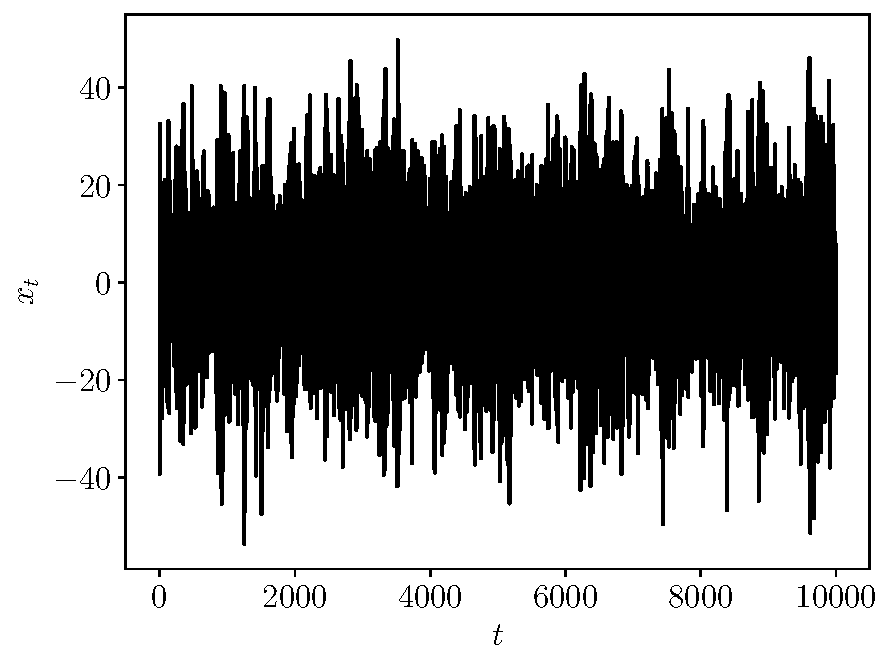
\includegraphics[scale=0.6]{figs/ts.pdf}
    \caption{Time series data.}
    \label{fig:ts}
\end{figure}
\end{enumerate}

The series was then tested for the stationarity, using the Augmented Dickey-Fuller (DF) test, the Philips-Perron (PP) test and the Kwiatkowski-Phillips-Schmidt-Shin (KPSS) test. Note that the DF and KPSS tests require the number of lags as an input parameter, therefore an appropriate number of lags must be selected before running the tests. The number of lags was selected based on the results obtained from the autocorrelation function (ACF) and partial autocorrelation function (PACF). The code to obtain the plots of these functions is:
\begin{minted}{python}
import statsmodels.api as sm

if plot:
    sm.graphics.tsa.plot_acf(data, lags=25, title='')
    plt.savefig('figs/acf.pdf', bbox_inches='tight')
    plt.clf()
    sm.graphics.tsa.plot_pacf(data, lags=25, title='')
    plt.savefig('figs/pacf.pdf', bbox_inches='tight')
\end{minted}
The obtained plots are presented in Figure \ref{fig:cf}. Note that the ACF shows an exponential decay with significant values along most the lags. The PACF, however, shows significant values at the beginning and it vanishes abruptly after 12 lags; showing that the process behind the series data is highly autocorrelated at most for 12 lags. These facts can be used as strong evidence of the model having, at least, an AR(12) process within. Additionally, the ACF plot does not show a significant decrease in the first 100 lags, suggesting that the MA process is either of really high order (which is unlikely) or it is an MA(0) process. Hence the tests were executed with 12 lags.

\begin{figure}[H]
    \centering
    \begin{subfigure}[b]{0.45\textwidth}
        \centering
        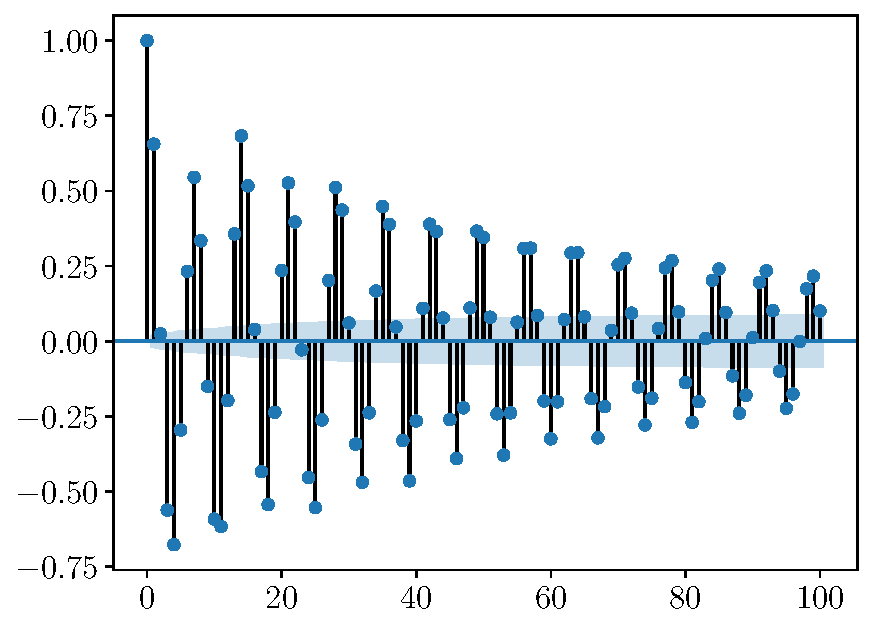
\includegraphics[width=\textwidth]{figs/acf.pdf}
        \caption{Autocorrelations.}
        \label{fig:acf}
    \end{subfigure}
    \begin{subfigure}[b]{0.45\textwidth}  
        \centering 
        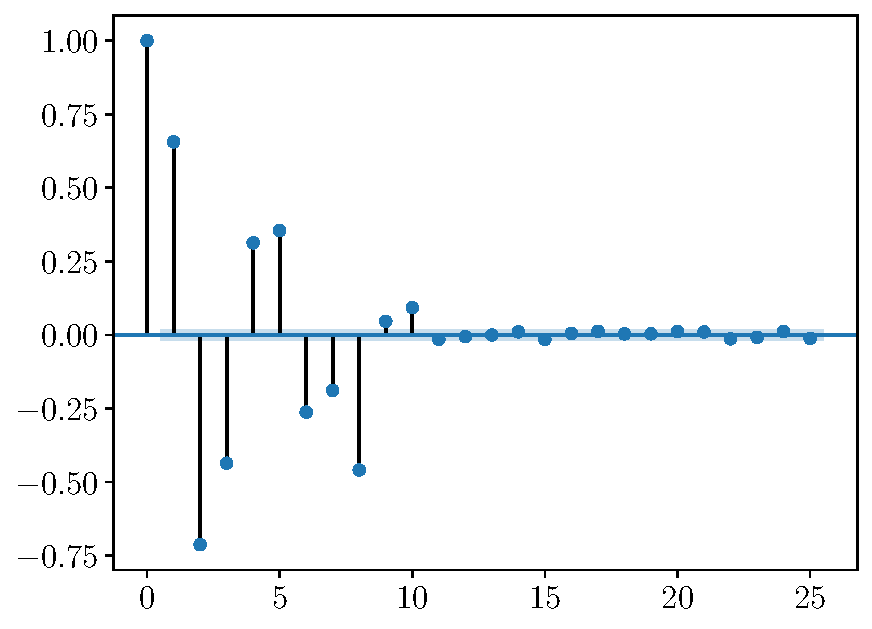
\includegraphics[width=\textwidth]{figs/pacf.pdf}
        \caption{Partial Autocorrelations.}
        \label{fig:pacf}
    \end{subfigure}]
    \caption{Estimated Autocorrelation Functions.}
    \label{fig:cf}
\end{figure}

The obtained p-values for these tests are presented in Table \ref{tab:pvals}. Recall that the DF and PP test under the null hypothesis that there exists an unitary root and hence the series is not stationary, while the KPSS test under the null hypothesis that the series is stationary. Let us present the code to obtain the tests results:
\begin{minted}{python}
from arch.unitroot import PhillipsPerron

# Dickey-Fuller
outDF = sm.tsa.stattools.adfuller(data, 12, regression='nc')
print('p_val DF:', outDF[1])

# KPSS
outKPSS = sm.tsa.stattools.kpss(data, nlags=12)
print('p_val KPSS:', outKPSS[1])

# Phillips - Perron
print('p_val PP:', PhillipsPerron(data).pvalue)
\end{minted}

\begin{table}[H]
\centering
\caption{Stationarity tests results.}
\label{tab:pvals}
\begin{tabular}{ll}
\hline
\textbf{Test} & \textbf{p-value} \\ \hline
DF & 0.0 \\
PP & 0.0 \\
KPSS & $>$0.1 \\ \hline
\end{tabular}
\end{table}

Hence, taking into consideration the above comment on the null hypothesis of each test and the obtained p-values, it can be concluded that the time series data is stationary. Finally, with the discussion regarding Figure \ref{fig:cf}, and given that the series is stationary (an integrated process is not required), the model that is believed to fit the series data is an AR(12) process.

Then, the model was fitted using the Statsmodels library in Python. Additionally, the diagnostics of the fitting was also obtained and plotted. The code for this process is:
\begin{minted}{python}
# Estimate model
mod = sm.tsa.arima.ARIMA(data, order=(12, 0, 0))
res = mod.fit()
print(res.summary())

if plot:
    plt.clf()
    plt.rcParams.update({'font.size': 11})
    fig = res.plot_diagnostics()
    fig.tight_layout(pad=1.25)
    plt.savefig("figs/res.pdf")
\end{minted}

The fitting results are presented in Figure \ref{fig:fit} and the residual diagnostics are presented in \ref{fig:fit}. Note that the residual analysis results are consistent with the assumption of order zero for the MA process.

\begin{figure}[H]
    \centering
    \begin{subfigure}[b]{0.45\textwidth}
        \centering
        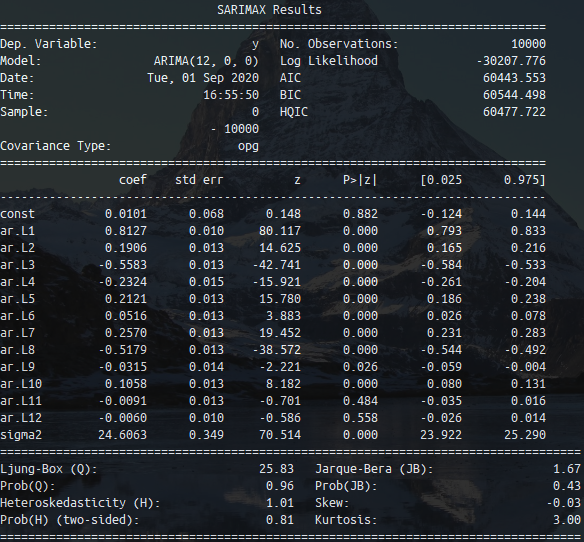
\includegraphics[scale=0.5]{figs/res.png}
        \caption{Fitting results.}
        \label{fig:fit}
    \end{subfigure}
    \begin{subfigure}[b]{0.45\textwidth}  
        \centering 
        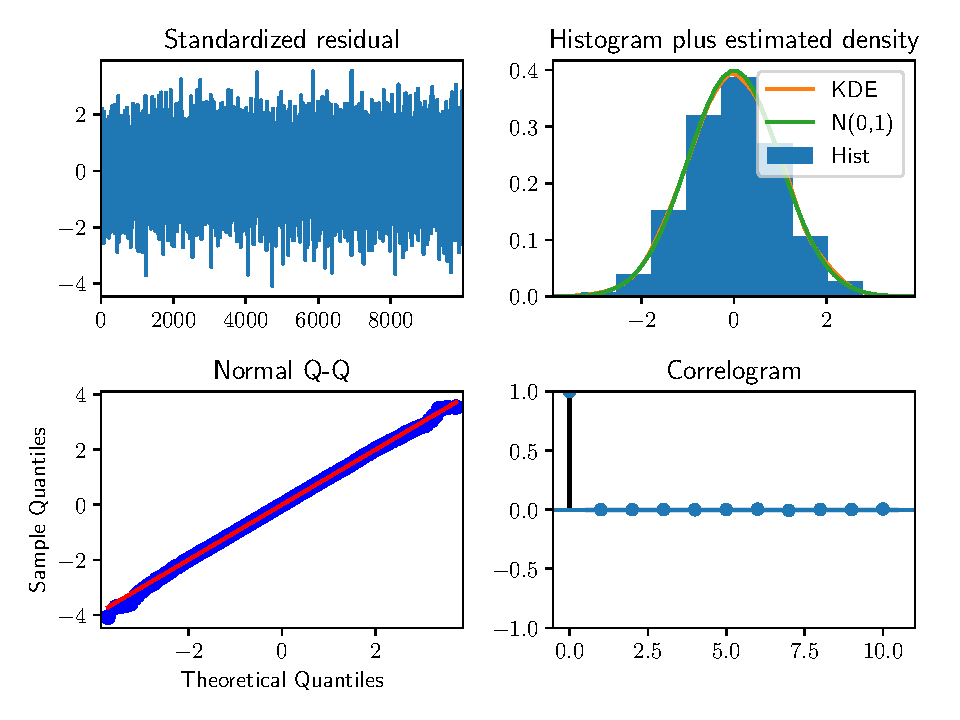
\includegraphics[width=1.35\textwidth]{figs/res.pdf}
        \caption{Residual analysis.}
        \label{fig:res}
    \end{subfigure}
    \caption{Fitting results.}
    \label{fig:ress}
\end{figure}

% \bibliographystyle{IEEEtran}
% \bibliography{bibs}
\end{document}
